\documentclass[11pt, a4paper]{article}
\usepackage{ifxetex}
\usepackage{amsmath}
\usepackage{hyperref}

\ifxetex
	\usepackage{fontspec}
	\usepackage{unicode-math}
	\setmainfont[Ligatures=TeX,
		Extension=.otf,
		BoldFont=*-bold,
		UprightFont=*-regular,
		ItalicFont=*-italic,
		BoldItalicFont=*-bolditalic,
	SmallCapsFeatures={Letters=SmallCaps}]{texgyrepagella}
	\setmathfont[Ligatures=TeX]{texgyrepagella-math.otf}
	
	% set up Heros (Helvetica)
	\setsansfont[Ligatures=TeX,
		Extension=.otf,
		BoldFont=*-bold,
		UprightFont=*-regular,
		ItalicFont=*-italic,
		BoldItalicFont=*-bolditalic,
	SmallCapsFeatures={Letters=SmallCaps}]{texgyreheros}
\else
	\usepackage[utf8]{inputenc}
	\usepackage[T1]{fontenc}
\fi

\usepackage{ngerman}
\usepackage{booktabs}
\usepackage{microtype}

\usepackage{svg}
\usepackage{graphicx}
\graphicspath{{../img/}}

\title{Grapheigenschaften auf Kookkurrenzgraphen in Leichter und Standardsprache auf Wikipedia- und Nachrichtencorpora}
\author{Author 1, Author 2, Author 3\\Modul "`Fortgeschrittene Methoden des Information Retrieval"'}
\date{\today}

\begin{document}
\maketitle
\tableofcontents

\section{Motivation und Ziel}

Leichte oder auch Einfache Sprache ist eine Untermenge der deutschen Sprache,
die auf besonders leichte Verst\"andlichkeit optimiert ist. Sie umfasst unter
anderem spezielle Sprachregelungen, typographische Empfehlungen und
Rechtschreibregeln. 

Das \emph{Netzwerk Leichte Sprache} definiert folgende grundlegenden
Eigenschaften Leichter Sprache:

% Quellenangabe?!
\begin{itemize}
	\item Benutzen Sie einfache W\"orter
	\item Benutzen Sie W\"orter, die etwas genau beschreiben
	\item Benutzen Sie bekannte W\"orter und verzichten sie auf Fachw\"orter und Fremdw\"orter
	\item Benutzen Sie immer die gleichen W\"orter f\"ur gleiche Dinge
	\item Benutzen Sie kurze W\"orter
	\item Verzichten Sie auf Abk\"urzungen
	\item Benutzen Sie Verben
	\item Vermeiden Sie den Genitiv und Konjunktiv
	\item Vermeiden Sie Kolloquialismen und bildliche Sprache
	\item Benutzen Sie Ziffern anstatt von Worten
	\item Schreiben Sie kurze S\"atze, die nur eine Aussage enthalten
	\item Benutzen Sie einen einfachen Satzbau
	\item Schreiben Sie jeden Satz in eine Zeile
\end{itemize}

Das englische \"Aquivalent zu Leichter Sprache ist \emph{Simple English}. Es
existieren verschiedene Modelle des Simple English, welche unterschiedliche
Ziele erreichen sollen -- z.B. das \emph{Simplified Technical English}, eine
kontrollierte Sprache f\"ur technische Handb\"ucher. Aufgrund dieser
konkurrierenden Ans\"atze gibt es keine einheitliche Definition oder
Sprachpraxis des Simple English. So sind z.B. i TODO ???

\section{Tools}
\paragraph{Programmiersprache Python}
Nach sprachunanbängigen Recherchen über verwendbare Bibliotheken haben wir uns wegen der bereits implementierten Graphalgorithmen in \texttt{graph-tool} für die Programmiersprache Python\footnote{\url{https://www.python.org/}} entschieden. Wegen der Unicodeunterstützung wurde Python 3 gewählt.

\paragraph{Graphen-Bibliothek \texttt{graph-tool}}
\texttt{graph-tool}\footnote{\url{http://graph-tool.skewed.de/}} ist ein Python-Modul,
welches der Manipulation und statistische
Auswertung von Graphen dient. Es stellt im Kern ein C++-Wrapper um die Boost
Graph Library dar, wodurch eine \"ahnliche Performanz zu nativen C-Bibliotheken
erreicht wird. Es ist zus\"atzlich in der Lage, Graphen mit modernen Techniken
zu visualisieren und \"ubliche Ma\ss{}e wie Clustering-Koeffizienten, Knoten-
und Kantengrade und Durchmesser zu berechnen.

\paragraph{NLP-Framework NLTK}
Das Natural Language Toolkit (NLTK\footnote{\url{http://www.nltk.org/}}) ist ein Framework f\"ur Sprachverarbeitung in Python. Die verwendeten Stopwortlisten, sowohl für Deutsch, als auch für Englisch stammen aus der Bibliothek.

\section{Datenbasis}

Als Datenbasis wurden Quellen gew\"ahlt, die sich durch eine gro\ss{}e
semantische und logische N\"ahe auszeichnen, namentlich Nachrichtenseiten in
deutscher und Wikipediaartikel in englischer Sprache.

\subsection{Nachrichtenseiten}

\subsubsection{nachrichtenleicht.de (nl)}

Nachrichtenleicht ist ein Dienst des Deutschlandfunks, welcher einmal
w\"ochentlich die wichtigsten Nachrichten der vorangegangenen Woche in Leichter
Sprache zusammenfasst. Er soll die mehreren Millionen Menschen in Deutschland
erreichen, die aus verschiedenen Gr\"unden von konventionellen
Nachrichtenangeboten ausgeschlossen sind.

\subsubsection{deunews2010\_100K Corpus der ASV (denews10k)}

Als korrespondierende Datenquelle in Standardsprache wurde der
deunews\-2010\_100K-Corpus des Lehrstuhls f\"ur automatische Sprachverarbeitung
der Universit\"at Leipzig gew\"ahlt. Dieser weist eine \"ahnliche Satzzahl zu
den von nachrichtenleicht extrahierten Text aus und wurde bereits von der ASV
normalisiert.

\subsection{Wikipedia (wiki\_sim bzw. wiki\_en)}

Die zweite Datenquelle sind Artikel aus der Wikipedia in \emph{Simple} und
\emph{Standard English}. Mit fast 120.000 Lemmata stellt die Simple English
Wikipedia eine der gr\"o\ss{}ten \"offentlich frei verf\"ugbaren Textsammlungen
in einer einfachen Sprachvariante dar. Zus\"atzlich ist sie die
einzige, welche Dokumentenalignment aufweist, was die einfache Erstellung zwei
inhaltlich homogener Corpora gestattet.

\section{Workflow}
\subsection{Datenextraktion und Erstellung der Corpora}

Mittels selbstgeschriebener Crawler wurden die relevanten Textmengen
heruntergeladen, extrahiert und zu Corpora zusammengefasst.

Nachrichtenleicht wurde rekursiv von der Startseite gequeriet
und die resultierenden Texte in einer MongoDB gespeichert.
Dabei wurden Überschriften, Teaser und Nachrichtentext jeweils seperat erfasst
und schließlich Teaser und Nachrichteninhalt zum Corpus hinzugefügt.

Zur Erstellung der Wikipedia-Corpora wurde zunächst eine Liste aller
in Simple English verfügbaren Artikel erstellt. Anschließend wurden diese und
die jeweils korrespondierenden Artikel in Standard English heruntergeladen und
im Rohformat (mit eingebettetem MediaWiki-Markup) in einer JSON-Datei gespeichert.
\\
Die Entfernung des Markups stellte sich als eine nichttriviale Aufgabe dar.
Der vollständige MWParser\footnote{MediaWiki
Parser from Hell (\url{http://mwparserfromhell.rtfd.org})} erwies sich für die
entsprechende Datenmenge (ca. 2 GB Dateigröße des Dumps) als deutlich zu langsam
und somit unbrauchbar.
\\
Mit einem Python-Skript, das Markup mit Hilfe regul\"arer Ausdr\"ucke entfernt
bzw. umwandelt, konnten jedoch zufriedenstellende Ergebnisse mit vertretbarem
Zeitaufwand erzielt werden.
Nach Entfernen des Wiki-Markups wurden die Artikel auf die Satzanzahl
des jweils k\"urzeren Artikels reduziert und anschliessend in einer MongoDB
gespeichert.

\subsection{Berechnung der Kookkurrenzen}

Die Kookkurrenzen wurden von mittels der Pipeline des Lehrsstuhls f\"ur
Automatische Sprachverarbeitung für uns berechnet und in eine MySQL-Datenbank
gespeichert.

\subsection{Erstellung der Graphen}

Die errechneten Kookkurrenzen wurden in \texttt{graph-tool}-Objekte geparst. Subgraphen
aus den Corpora wurden mittels eines \texttt{force-directed graph} nach
\cite{Hu2005} gelayoutet.
Die relevanten Daten zur Erstellung der Histogramme wurden gespeichert,
um sie anschließend nach R zu exportieren und dort mittels ggplot2 zu plotten.

\subsection{Berechnung von Graphen-Kenngr\"o\ss{}en}

Nach Erstellung der Graphen wollen wir sie auf typische Kenngrößen untersuchen,
anhand dieser charakterisieren sowie paarweise vergleichen. Für die
verschiedenen Eigenschaften bietet \texttt{graph-tool} bereits implementierte
Algorithmen an, die wir verwenden wollen. Im Folgenden werden die Kenngrößen
kurz erläutert, unsere Erwartungen dargestellt und die Ergebnisse gezeigt.

\paragraph{Gr\"o\ss{}e (Knotenzahl)}

Schon in der Größe der Graphen sollten sich paarweise Unterschiede erkennen
lassen. So sollten die beiden Corpora in einfacher Sprache wesentlich weniger
verschiedene Wörter enthalten. Durch die Praxis, \emph{schwierige} Wörter
durch leichter verständliche zu ersetzen, ist zu erwarten, dass erstere im einfachen
Corpus nicht vorkommen. Die Anzahl der Knoten (ohne Stopw\"orter\footnote{Es wurde
die deutsche bzw. englische Stopwortliste des NLTK benutzt. Erg\"anzt wurde
diese durch das Wort "'dass"' in neuer Rechtschreibung}) lässt sich natürlich
trivial zählen. Der \emph{deunews2010\_100K-Corpus} hat 3205 respektive 1812
Knoten, \emph{nachrichtenleicht.de} 2946 (2305), die englische Wikipedia 45897
(39212), und die \emph{simple english} Wikipedia 36582 (31045) Knoten. In der
Tat l\"asst sich also schlie\ss{}en, dass diese grundlegende Erwartung
erf\"ullt ist. Des weiteren zeigt sich, dass keine bedeutsamen Unterschiede im
Anteil der Stopw\"orter zwischen den Corpora auftreten.

\paragraph{Rang der Kantengewichte}

TODO: Aussage verifizieren

Die Kantengewichte folgen dem zipfschen Gesetz wobei sich f\"ur Leichte Sprache
feststellen l\"asst, dass die Verteilung gleichm\"a\ss{}iger ist, d.h. weniger
Spezialvokabular im "'Long Tail"' der Verteilung auftritt.

\paragraph{Dichte}

Die Dichte eines Graphen beschreibt das Verhältnis von vorhandenen Kanten zu
potentiell möglichen Kanten in einem Graphen. Ein Wert von $1$ bedeutet, dass
jeder Knoten mit jedem anderen Verbunden ist, dem gegenüber eine $0$, dass keine
Kanten vorhanden sind. Die Dichte wird wie folgt berechnet:

$$
    \frac{|E|}{|V|(|V|-1)}
$$

$|E|$ ist die Anzahl der Kanten, $|V|$ die Anzahl der Knoten im Graphen. 

TODO: ist es hier plausibel, dass die einfachen sprachen dichter sein sollten?
es gibt ja (hoffentlich) weniger wörter, und diese wenigen sollten
dementsprechend häufiger verwendet werden und sich untereinander so leichter
verknüpfen.

Für die einfachen Sprachvarianten sollten die Graphen dichter sein als für
Standardsprache.
Wie bereits beschrieben, gibt es in ersteren weniger Vokabular, dementsprechend
weniger Knoten, die verbunden werden können. Die Vorhandenen kommen jedoch öfter 
gemeinsam vor und sind enger Verknüpft. Die Ergebnisse in Tabelle \ref{density_table}
zeigen genau dies. Der Nachrichtenleicht-Corpus ist über 31\% dichter als denews10k.
Bei den englischen Corpora beträgt der Unterschied knapp über 17\%

\begin{table}[h]
  \centering
  \begin{tabular}{l|l}
    Corpus            & Dichte          \\
    \hline
    nl                &  		0,0013148876 \\
    denews10k         &  		0,0009998379 \\
    wiki\_sim         &  		0,0002469035 \\
    wiki\_en          &  		0,0002109985 \\
  \end{tabular}
  \caption{\label{density_table} Die Graphdichten der Corpora}
\end{table}

\paragraph{Clusterkoeffizient}

Eng mit der Dichte verwandt ist der Clusterkoeffizient. Er beschreibt die
Anzahl vorhandener Dreiecke im Graph im Verhältnis zu möglichen Dreiecken. Drei
Knoten, die jeweils paarweise verbunden sind, bilden ein Dreieck. Ziel ist ein
Messwert der Aussagt wie sehr die Knoten Cliquen bilden. Lokal betrachtet
bedeutet der Wert die Wahrscheinlichkeit die Nachbarn eines Nachbarn zu kennen.
Da wir die Graphen global miteinander vergleichen möchten verwenden wir den
globalen Clusterkoeffizienten $C$. Er berechnet sich wie folgt:

$$
    C = \frac{3*\text{Anzahl der Dreiecke}}{\text{Anzahl verbundener Tripel}}
$$

Ein Tripel bezeichnet drei miteinander Verbundener Knoten, nicht
notwendigerweise ein Dreieck. Knoten A kann mit Knoten B und C verbunden sein,
während B nicht mit C verbunden ist. In \emph{Small-World-Graphen} ist dieser
Wert typischerweise hoch. 


% wir können für ausgewählte wörter vielleicht noch lokale clusterkoeffizienten
% berechnen, vielleicht für die besonders hoch verbundenen? sollten diese dann
% relativ klein sein? weil hubs ja verschiedene "teilgraphen" miteinander
% verbinden

% \paragraph{(Pseudo-)Diameter}
% \paragraph{K\"urzeste Wegl\"ange}
% die beiden fasse ich im folgendem punkt zusammen

\paragraph{Wegl\"angen}
Um Small-World-Eigenschaften nachzuweisen, ist es außerdem interessant, die
Weglängen im Graphen zu untersuchen. Eine gute Kenngröße ist dabei der Durchmesser
des Graphen, also der längste kürzeste Weg zwischen zwei Knoten. In einer
\emph{small-world} sind alle Knoten von allen anderen in wenigen Schritten
erreichbar, typischerweise in 5 bis 7 Schritten. \texttt{graph-tool}
erlaubt zum einen die Ausgabe eines Durchmessers, wie oben beschrieben, und zum
anderen die Ausgabe eines Histogramms, welches die Vorkommen der Längen aller
kürzesten Wege zeigt.

\begin{table}[h]
  \centering
  \begin{tabular}{l|llllllllll}
    Corpus      & 1      & 2      & 3       & 4       & 5       & 6      & 7      & 8             & 9             & 10           \\
\hline
    wiki\_en    & 0,04 & 5,3  & 47,36 & 41,43 & 5,5   & 0,34 & 0,01 & $\sim$0  & $\sim$0  & 0          \\
    wiki\_sim   & 0,05 & 6,01 & 47,77 & 40,2  & 5,6   & 0,36 & 0,01 & $\sim$0  & $\sim$0  & 0          \\
    nl          & 0,26 & 4,71 & 27,71 & 44,18 & 18,32 & 3,98 & 0,73 & 0,1         & $\sim$0  & $\sim$0 \\
    denews10k   & 2,0    & 3,21 & 19,19 & 44,26 & 25,31 & 6,6  & 1,11 & 0,11        & 0,01        & $\sim$0 \\
  \end{tabular}
  \caption{Anteile der Weglängen paarweiser kürzester Wege zwischen allen Knoten, in Prozent}
\end{table}

TODO, folgenden abschnitt an tatsächliche ergebnisse anpassen 

In der Tat können wir die Schrittzahl bestätigen, beispielsweise für den
nachrichtenleicht-Corpus haben wir einen Durchmesser von 6, und von
allen paarweisen Pfaden kommt dieser sehr selten vor. Bei XXX Knoten gibt
es YYY Pfade zu berechnen. Die meisten Knoten sind in drei bis vier Schritten
miteinander verbunden.
Das gleiche Bild zeigt sich bei den englischen Wikipedia-Corpora. Sowohl in 
Simple als auch in Standard English sind über 90\% der paarweisen
kürzesten Strecken vier oder weniger Schritte lang. Es gibt in beiden Fällen 
einige wenige Paare, die bis zu neun Sprünge auseinander liegen.
TODO Welche sind das? stammen die womöglich von alle von wenigen einzelnen wörtern? evtl rechtschreibfehler? 

                             
\paragraph{Skalenfreiheit}
Skalenfreie Graphen zeichnen sich duch exponential verteilte Knotengrade aus. Es gibt wenige Knoten mit sehr vielen Nachbarn, sogenannte \emph{Hubs}. Dem gegenüber haben die anderen Knoten relativ wenige Nachbarn. 

haben wir so etwas? wir können das mit \texttt{graph-tool} über die
clustering algorithmen leicht ausrechnen!  skalieren die graphen paarweise um
ein paar knoten, oder kommen neue wichtige (hubs) wörter hinzu?

\paragraph{Small World Eigenschaften}
Zusammengefasst zeichnen sich Small-World-Graphen durch kleine Durchmesser und
hohe Clusterkoeffizienten aus. Skalenfreiheit ist nicht zwangsläufig wichtig.
Wir konnten sowohl die kurzen Weglängen, als auch hohe Clusteringkoeffizienten
für alle Graphen nachweisen. TODO passt das? skalenfreiheit? 


\paragraph{Übersichtstabelle}
\section{Ergebnisse}
\subsection{Weitere Beobachtungen}
\paragraph{H\"aufigste W\"orter nach Sprache}

%%%%%%%%%%%%%%%%%%%%%%%%%%%%%%%%%%%%%%%%%%%%%%%%%%%%%%%%%%%%%%%%%%%%%%%%%%%%%%%%
\section{Testkapitel mit Testgrafiken}
Zur Erzeugung der Grafiken wurde der Threshold auf 100 erhöht, damit unwichtige Kanten die Grafiken nicht überladen.
TODO: Threshold je nach Corpus verschieden

\subsection{pdf-Grafik}
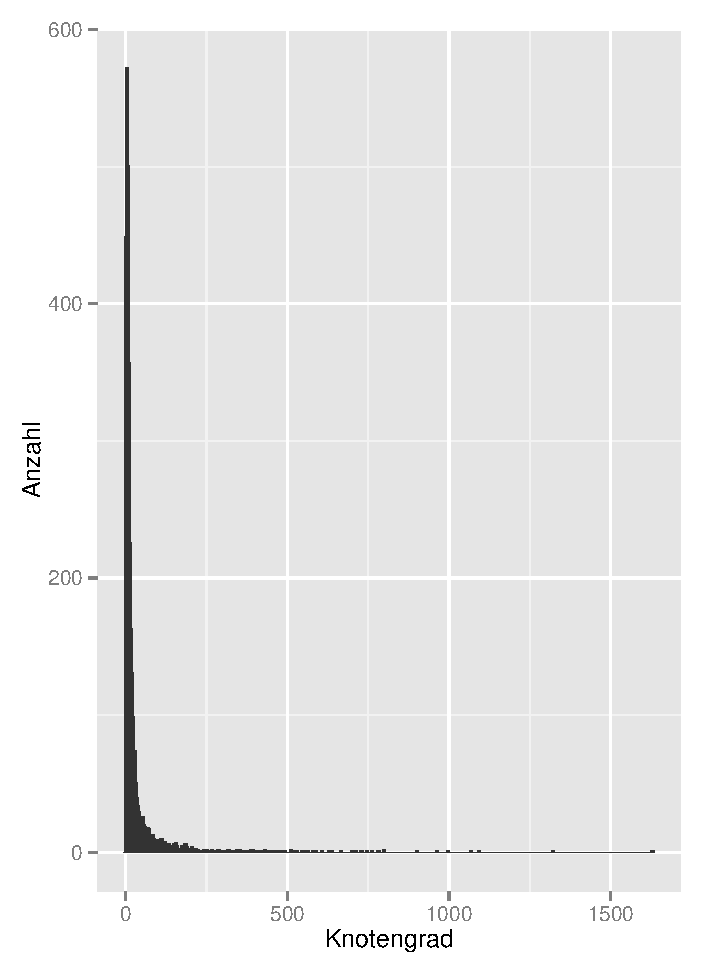
\includegraphics{testplot.pdf}

%%%%%%%%%%%%%%%%%%%%%%%%%%%%%%%%%%%%%%%%%%%%%%%%%%%%%%%%%%%%%%%%%%%%%%%%%%%%%%%%

\newpage
\begin{thebibliography}{9}
	\bibitem{Hu2005} Yifan Hu, Efficient and High Quality Force-Directed Graph, Mathematica Journal, vol. 10, Issue 1, pp. 37-71, (2005)
        \bibitem{Newman2003} Newman, Mark EJ. "The structure and function of complex networks." SIAM review 45.2 (2003): 167-256.
\end{thebibliography}
\end{document}
